\documentclass{bucthesis}
\begin{document}

%---------------------------------------------------------------------------%
%->> Personal information,个人信息
%---------------------------------------------------------------------------%
\institute{机电工程学院}
\major{机电工程实验班}
\class{机实1601}
\studentid{2016000000}
\title{基于\LaTeX{}排版的北京化工大学本科\\毕业设计论文模板}
\titleen{BEIJING UNIVERSITY OF CHEMICAL TECHNOLOGY UNDERGRADUATE GRADUATION DESIGN THESIS TEMPLATE BASED ON LATEX TYPESETTING}
\author{独小凡}
\teacher{独\hspace{1em}凡}
%---------------------------------------------------------------------------%
%->> Cover & Statement,封面诚信申明
%---------------------------------------------------------------------------%
\maketitle%生成封面
%\pdfbookmark[0]{封面}{title}  
\frontmatter%诚信申明
%---------------------------------------------------------------------------%
%->> Abstract & Keywords,中文摘要&关键词
%---------------------------------------------------------------------------%
\abstractzh{\par
	本文是北京化工大学学位论文\LaTeX{}模板{~\textbf{bucthesis}~}\upcite{bucthesis}的使用说明,用例子展示模板的使用方法;用论文撰写规范填充无关紧要的部分;对照文档注释以及本文档使用会有奇效。\par
	摘要是学位论文的内容不加注释和评论的简短陈述。置于诚信声明后。摘要应具有独立性和自含性,即不阅读论文的全文,就能获得必要的信息。摘要中有数据、结论,是一篇完整的短文,可以独立使用和引用。摘要的内容应包含与论文正文等同量的主要信息,供读者确定有无必要阅读全文,也可供二次文献(文摘等)采用。摘要一般应说明研究工作的目的、实验方法、结果和最终结论等,重点突出具有创新性的成果和新见解。\par
	中文摘要一般为300字左右,英文摘要为1500印刷符号左右,含中、英文摘要关键词。英文摘要应与中文摘要内容一致。除非无法变通的办法可用以外,摘要中不用图、表、化学结构式、非公知公用的符号和术语。\par
	关键词是为了文献标引而从学位论文中选取出来用以表示全文主题内容信息款目的单词或术语。关键词用显著的字符另起一行,排在摘要的左下方。关键词一般不超过3个。\par}
	{北京化工大学,学位论文,\LaTeX{}模板}
%---------------------------------------------------------------------------%
%->> Abstract & Keywords,英文摘要&关键词
%---------------------------------------------------------------------------%
\abstracten{\par
	This article is an instruction for the use of the degree thesis \LaTeX{} template {~\textbf{bucthesis}~} of Beijing University of Chemical Technology, using examples to show how to use the template; filling in the irrelevant parts with the paper writing specifications; comparing the documentation comments and the use of this document There will be wonders. \par
	The abstract is a short statement without comments and comments on the content of the dissertation. After the integrity statement. The abstract should be independent and self-contained, that is, the necessary information can be obtained without reading the full text of the paper. The summary contains data and conclusions, and is a complete short article that can be used and quoted independently. The content of the abstract should contain the same amount of main information as the body of the paper, for readers to determine whether it is necessary to read the full text, or for secondary literature (abstract, etc.). The abstract should generally explain the purpose of the research work, experimental methods, results and final conclusions, etc., focusing on innovative results and new insights. \par
	The Chinese abstract is generally about 300 words, and the English abstract is about 1500 printed symbols, including keywords in Chinese and English abstracts. The English abstract should be consistent with the Chinese abstract. Unless there are no alternatives available, the abstract does not use figures, tables, chemical structural formulas, or symbols or terms that are not publicly known. \par
	The key words are words or terms that are selected from the dissertation for the purpose of document indexing to represent the full-text subject content information items. Key words start on a new line with prominent characters and are listed at the bottom left of the summary. There are generally no more than 3 keywords.}
	{Beijing University of Chemical Technology(BUCT), degree thesis, \LaTeX{} template}

%---------------------------------------------------------------------------%
%->> Table of Contents,目录
%---------------------------------------------------------------------------%
\tableofcontents%目录
%\pdfbookmark[0]{目录}{toc}
%\addcontentsline{toc}{section}{目录}%将目录加入到目录

%---------------------------------------------------------------------------%
%->> Symbol Description,符号说明
%---------------------------------------------------------------------------%
\symbolpage{
	\begin{table}[h]
		\raggedright
		\zihao{4}
		\renewcommand\arraystretch{1.5}
%		\resizebox{\textwidth}{!}{%
			\begin{tabular}{p{6em}l}
				\LaTeX{} & 基于\TeX{}的排版系统 \\ 
				BUCT     & 北京化工大学         \\ 
				awsl     & 表示XX太可爱,啊我死了     \\ 
			\end{tabular}%
	\end{table}}

%---------------------------------------------------------------------------%
%->> Main Body,正文
%---------------------------------------------------------------------------%
\startmain
\chapter{作者声明}{\zihao{3}\par
	\LaTeX{}以及本模板在上手时会有一定的难度,因此不能保证所有人能顺利使用。\par
	本模板未经过全平台测试,未经过全情况测试,可能存在潜在的Bug,欢迎反馈但\textbf{不能}保证修复。\par
	本模板某些方面不满足相关要求,故使用本模板造成(包括但不限于)论文审核不通过等所有问题作者概不负责,请根据自身情况决定是否使用。\par
	本项目为兴趣之作,已在\faGithubAlt{\textbf{\href{http://www.github.com}{GitHub}}} 开源,喜欢本项目的欢迎Star支持。\par
%	由于精力有限,不能保证后续更新。\par
	欢迎志同道合的人一起加入。\par
	}
\chapter{综述}{\par
	学位论文是取得学位的一个重要环节,但是这个环节往往是复杂而使人头秃\footnote{ltx如是说}的。如何快乐的完成学位论文成了众多学子日思夜想的问题。本模板将带你入坑并带你出坑,当然前提是你要自带内容,毕竟巧妇难为无米之炊嘛\footnote{谚语}。\par}
\section{快速开始}{\par
	此部分为了演示编号功能,具体使用参见第\ref{use}章。
	\begin{enumerate}[\hspace{2em}(a)]
		\item 安装\TeX{}发行版
		\item 下载本模板
		\item 在main.tex中编写,
		\item 编译
	\end{enumerate}}
\section{减轻的负担}{\par
	使用本模板可以大大减轻您论文的排版负担,而且将大部分的排版与内容分离,使您更能专注于内容,在保证写作效率的同时提高您的体验。}
\section{带来的麻烦}{\par
	您可能需要学习\LaTeX{}的基本操作,以及公式、表格、图片、代码等环境的使用,包括但不限于编译失败等其他衍生问题,若不熟悉\LaTeX{}则在一定程度上增加了写作难度,使用前请酌情考虑。\par}

\chapter{使用说明}{\par
	本模板需要\LaTeX{}环境,并且采用xelatex引擎编译。{\textbf{\href{http://tug.org/texlive/}{TexLive}}}是由国际TeX用户组织TUG开发的TeX系统,支持不同的操作系统平台。{\textbf{\href{https://miktex.org/}{MiKTeX}}}是Windows系统下的\LaTeX{}编译系统。请根据需要自行选择安装。}\label{use}

\section{文前}
\subsection{封面}{\par
	本模板中已经完成封面格式排版,只需将个人相关信息填写并编译即可生成封面。实际上封面由学校统一印制,所以本部分非必须,只是为了美观而存在。}
\subsection{诚信申明}{\par
	此部分不需要做任何更改。}
\subsection{摘要}{\par
	中英文摘要分别填写到\verb|\abstractzh{}{}|和\verb|\abstracten{}{}|的第一个大括号中即可。下面是中文摘要要求,用以展示文档中编号的用法。
	\begin{itemize}
		\item[*] 论文题目为三号黑体字,可以分成1或2行居中打印
		\item[*] 论文题目下空一行居中打印“摘要”二字(小三号黑体),两字间空一格(注:“一格”的标准为一个汉字,以下同)
		\item “摘要”二字下空一行,打印摘要内容(四号宋体)。段落按照“首行缩进”格式,每段开头空二格,标点符号占一格。
		\item 摘要内容后下空一行打印“关键词:”(四号黑体),其后为关键词(四号宋体)。关键词数量一般为3个,用“,”号分隔,句末不加标点。
	\end{itemize}
}

\subsection{关键词}{\par
	关键词一般不超过3个。中英文关键词分别填写到\verb|\abstractzh{}{}和\abstracten{}{}|第二个大括号中即可。}
\subsection{目录}{\par
	目录自动生成,无需做调整。}
\subsection{符号说明}{\par
	将相关内容填写到\verb|\symbolpage{}|中即可。}
\section{正文}
\subsection{标题}{\par
	用\verb|\chapter{title}|生成新的一章,title填对应的章标题即可。同理\verb|\section{title}|对应``条",\verb|\subsection{title}|对应``款",\verb|\subsubsection{title}|对应``项",使用方法同``章"。按照出现的顺序依次编号\upcite{刘海洋}。}
\subsection{图}{\par
	图已经设置好按章编号,如图\ref{fig:music}是一个图片示例,图\ref{fig:musictrim}是裁剪图片示例。\par	
	\begin{figure}[!htbp]
		\centering
		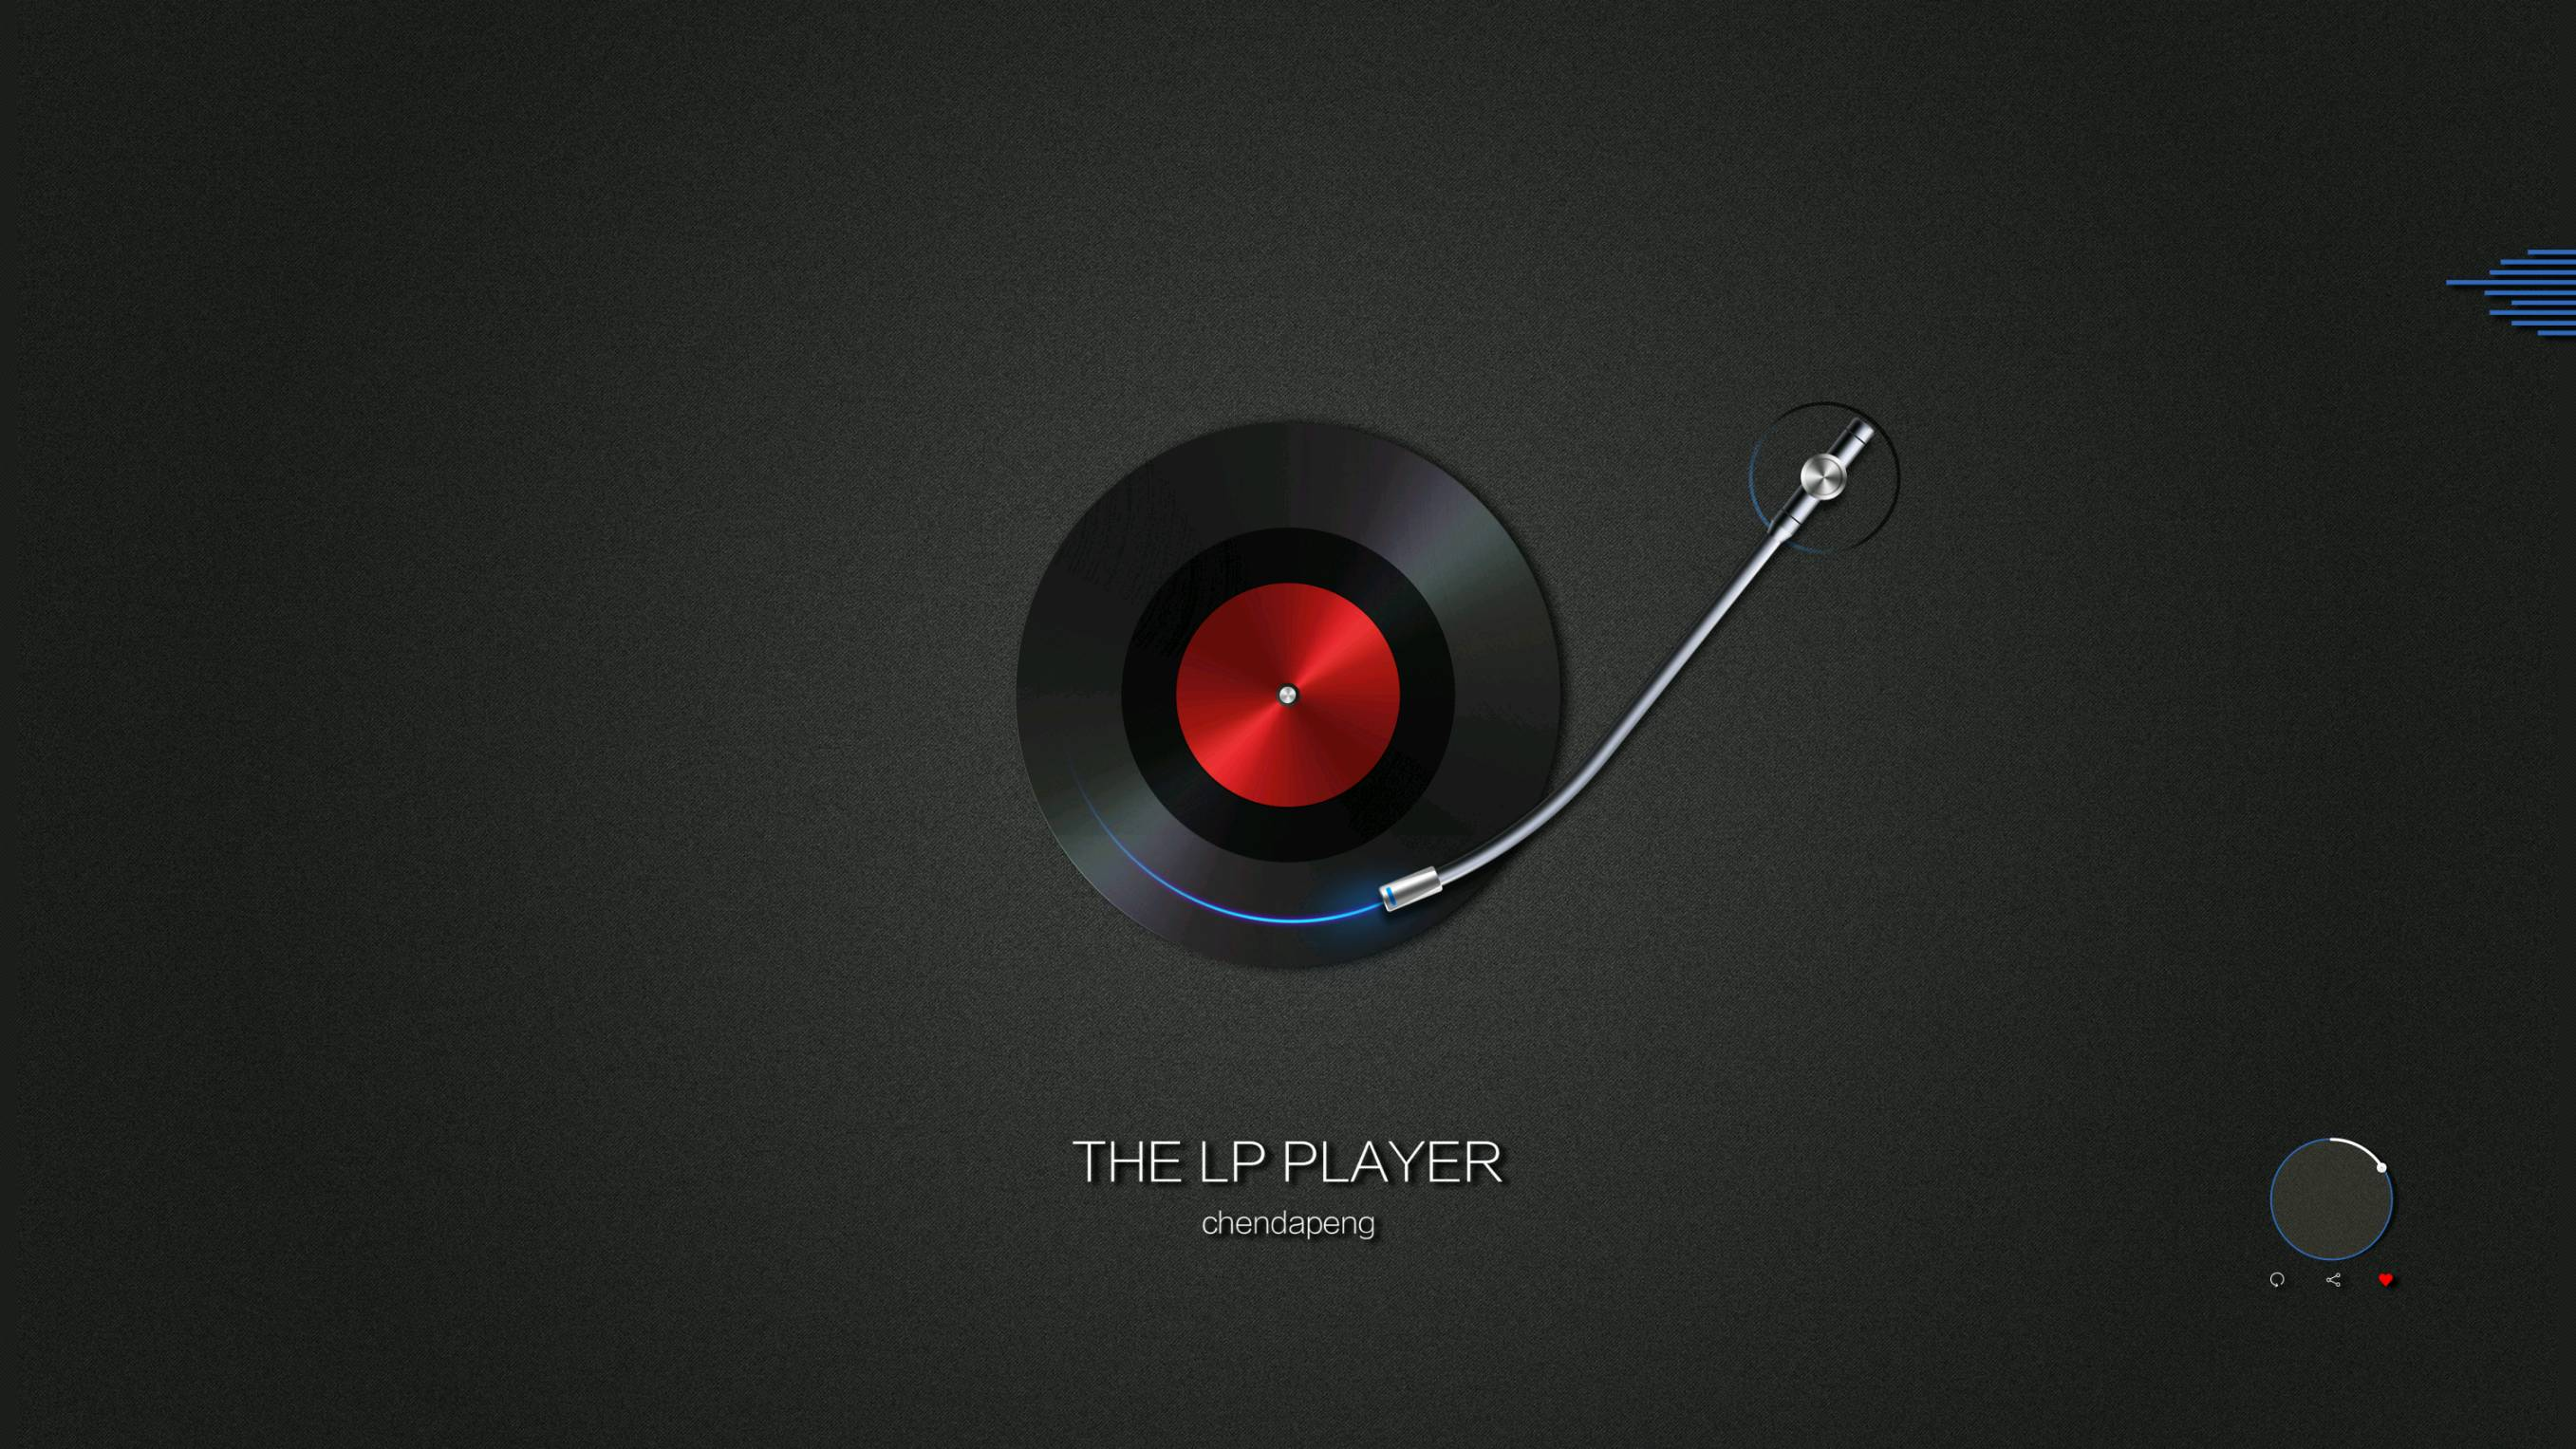
\includegraphics[width=0.8\linewidth]{image/music.jpg}\\
		\bicaption{图片示例}{music picture}
		\label{fig:music}
	\end{figure}
	
	\begin{figure}[!htbp]
		\centering
		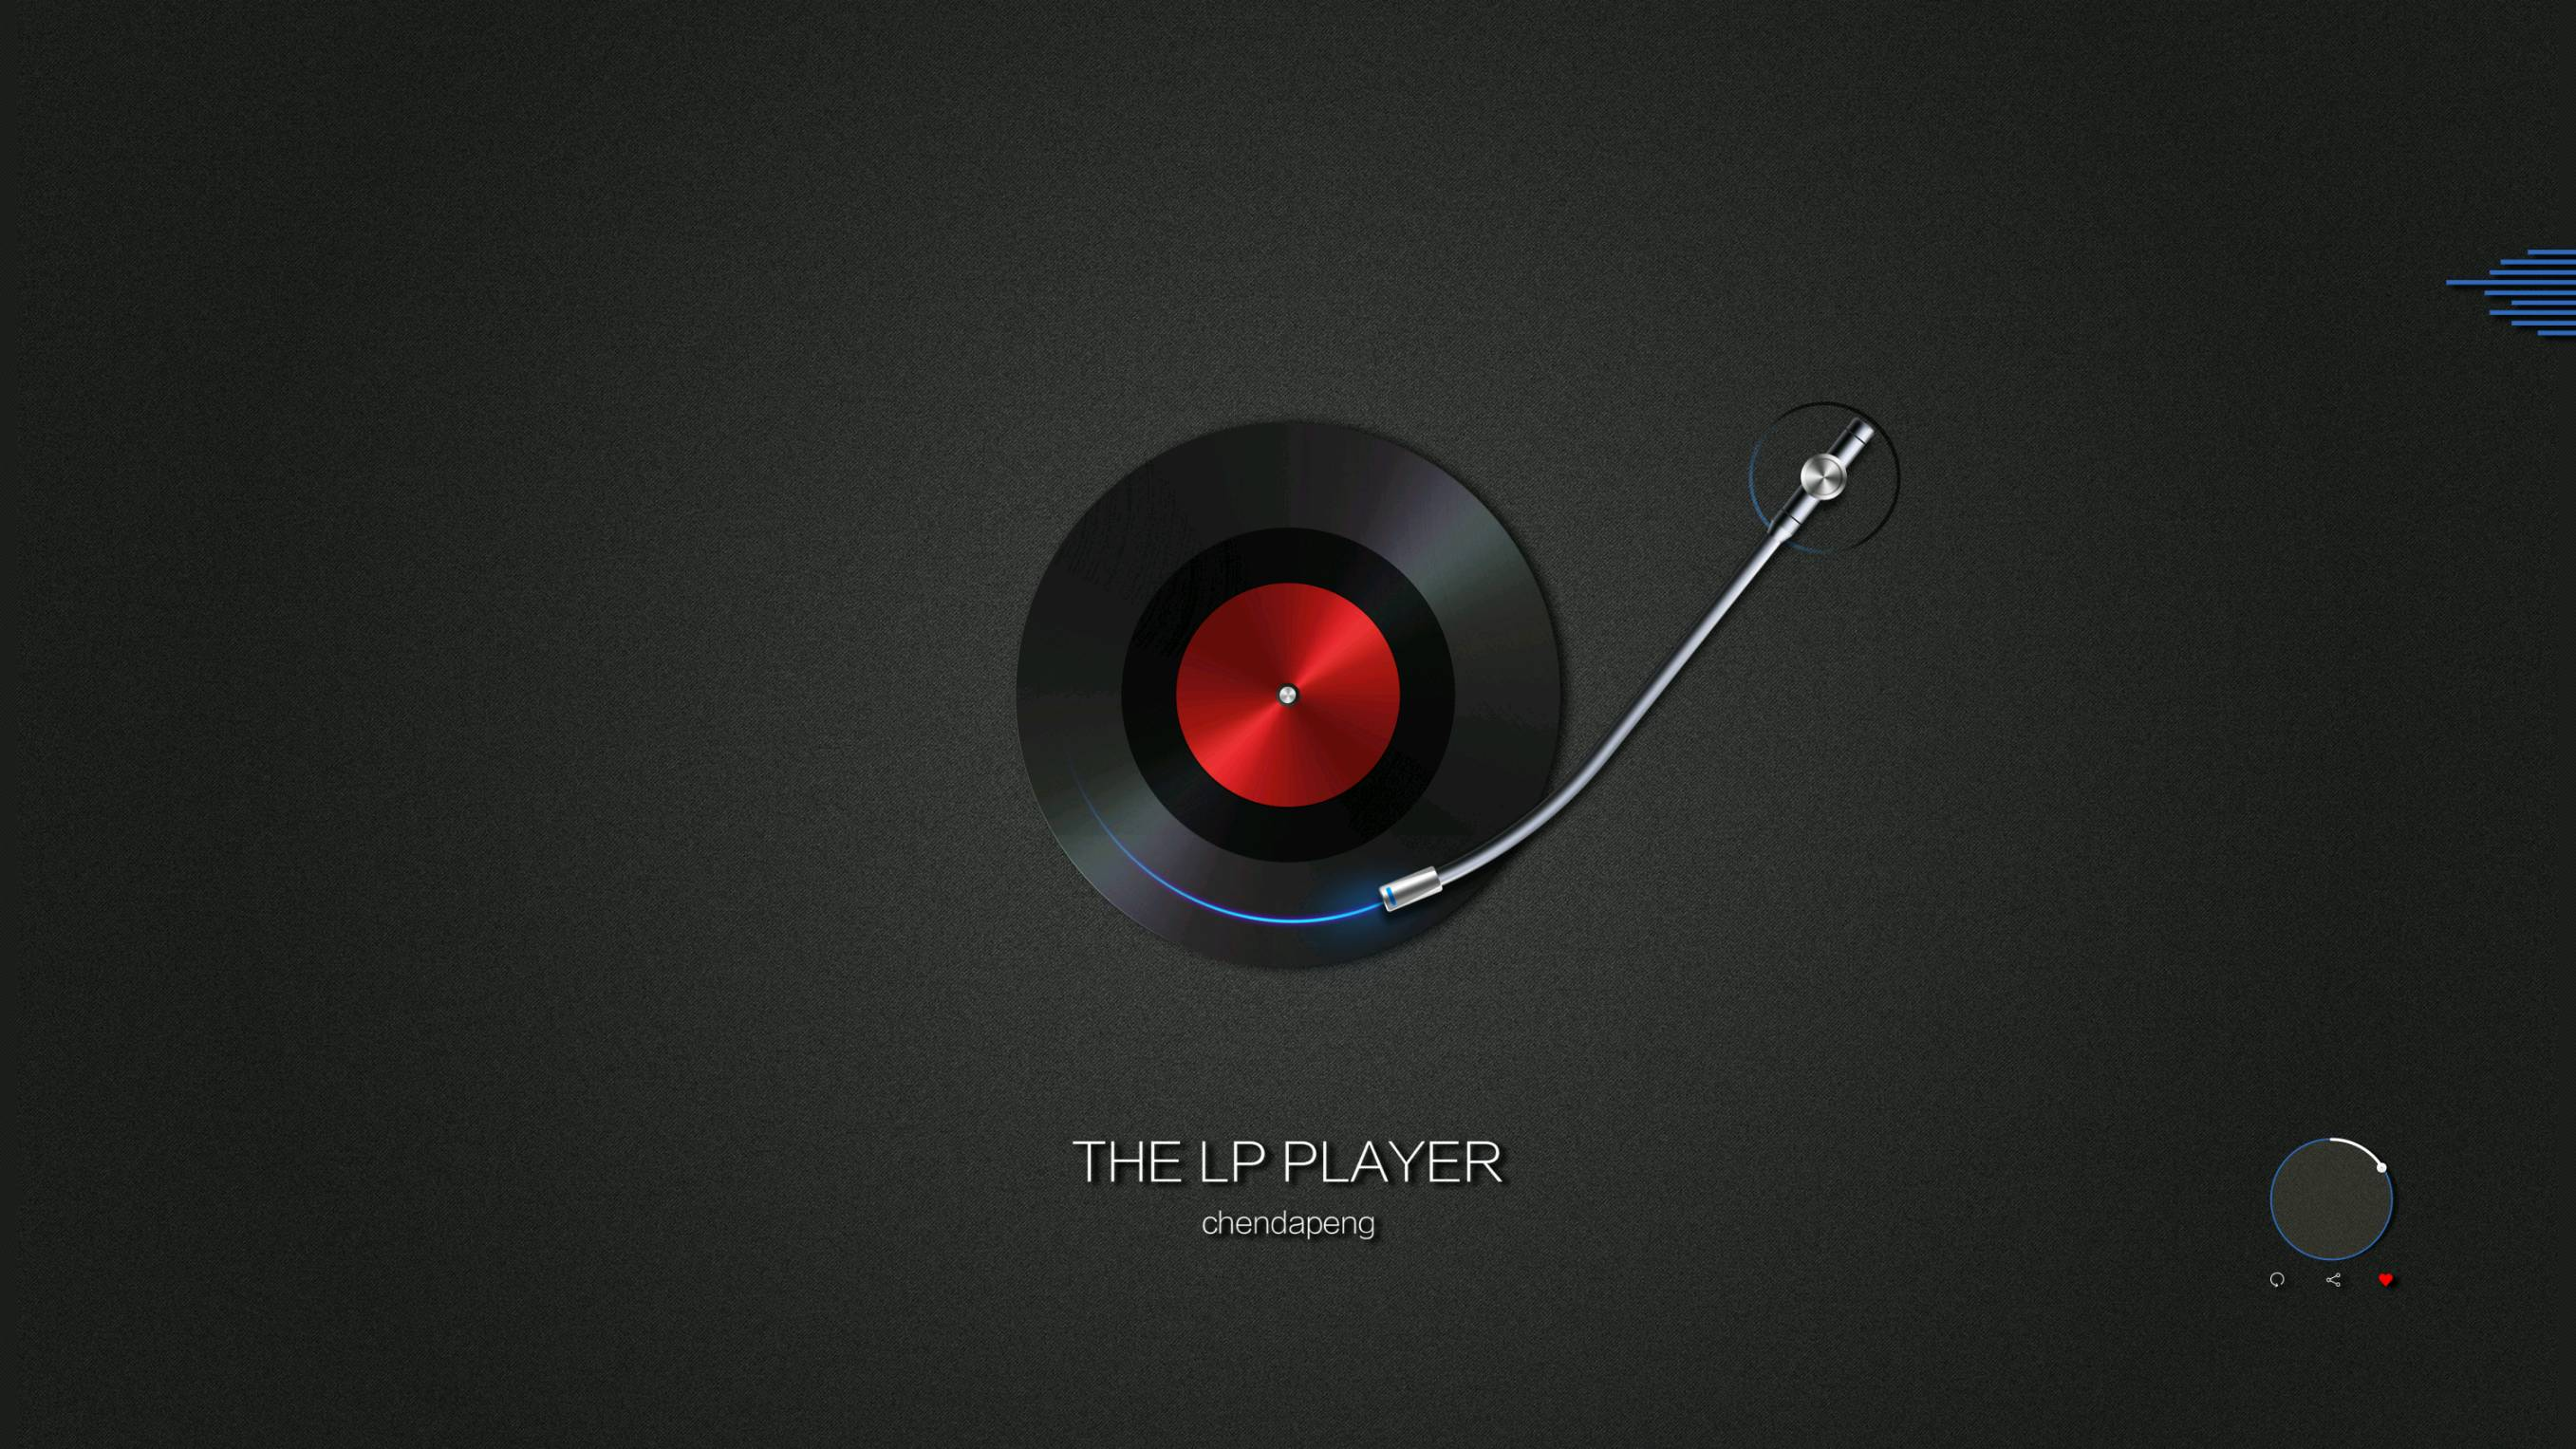
\includegraphics[trim=700 200 700 200,clip,scale=0.8,width=0.4\linewidth]{image/music.jpg}\\
		\bicaption{裁剪图片示例}{picture trimed}
		\label{fig:musictrim}
	\end{figure}
}
\subsection{表}{\par
	表已经设置好按章编号,如表\ref{tab:1}所示是一个简单表格示例。关于表格可以使用{https://www.tablesgenerator.com}这个网站可视化编辑表格并转换成\LaTeX{}代码插入文档使用。\par
	\begin{table}[ht]
		\centering
		\renewcommand\arraystretch{1.5}
		\bicaption{一般三线表}{General three-line table}
		\label{tab:1}
		\begin{tabular}{c c c| c c c c c c c c}
			\hline
			示例 & 1  & 2  & \multicolumn{8}{c}{跨列标题}\\
			\hline
			123 & 456 & 13 & 13 & 4 & 54 & 61 & 45 & 61 & 7 & 55\\
			133 & 456 & 7 & English & 4 & 61 & 61 & 57 & 61 & 102 & 57\\
			233 & 7 & 8 & 47 & 4 & 61 & 61 & 188 & 61 & 文字 & 61\\
			\hline
		\end{tabular}
	\end{table}}
\subsection{公式}{\par
	行内公式就像$a+b=c$这样,行间公式就像下面这样:
	\begin{equation}\label{equ1}
	\mbox{这是一个带编号的公式}\qquad
	a^2_{ij}+b^2_{ij}=c^2_{ij} \\[-2em]
%	\tag{\thechapter{}-\arabic{equation}}
	\end{equation}
	\begin{equation}
	\mbox{带编号的公式测试编号}\qquad
	a^2_{ij}+b^2_{ij}=c^2_{ij} 
	\end{equation}
	\[
	\text{这是不带编号的}\quad
	a^2_{ij}+b^2_{ij}=c^2_{ij}
	\]
}
	
\subsection{定理环境}{\par
	\begin{theorem}[勾股定理]
		若 $a,b$ 为直角三角形的两条直角边,$c$ 为斜边,那么 $a^2 + b^2 + c^2.$
	\end{theorem}
	\begin{definition}
		这是一个测试。This is a test。
	\end{definition}
	\begin{lemma}
		这是一个测试。This is a test。
	\end{lemma}
	\begin{inference}
		这是一个测试。This is a test。
	\end{inference}
	\begin{proposition}
		这是一个测试。This is a test。
	\end{proposition}
	\begin{example}
		这是一个测试。This is a test。
	\end{example}
	\begin{remark}
		这是一个测试。This is a test。
	\end{remark}
	\begin{proof}
		这是一个测试。This is a test。
	\end{proof}}
\subsection{代码}{\par
	\centering
	\begin{lstlisting}[language=Python]
	 for loopnum in lst:
	 	sum += lst[loopnum]
	\end{lstlisting}}

\section{文后}
\subsection{参考文献}{\par
	参考文献使用\verb|\upcite{}|来使参考文献以上标形式出现,用\verb|\cite{}|使其同行出现。文献内容存放于ref.bib文件中,可以在谷歌学术或百度学术中获得对应文章的BibTeX引用,存到此文件中即可引用。\par
	另外论文要求的文件貌似对参考文献的细节做了保姆级的演示,与国标不同,暂未核对。}
\subsection{附录}{\par
	附录一般作为学位论文主体的补充项目。主要包括:正文内过于冗长的公式推导;供读者阅读方便所需要的辅助性的数学工具或重复性数据图表;由于过分冗长而不宜放置在正文中的计算机程序清单;具有重要参考价值的资料;论文使用的缩写说明等。附录置于参考文献之后,其页码与正文连续编排。}
\subsection{致谢}{\par
	将内容填写到\verb|\acknowledgements{}|大括号内即可。\par}
\chapter{测试}{\par
	下面的公式用来测试不同章节间的编号以及引用,上一个公式在这里\ref{equ1}
	\begin{equation}
	a^2_{ij}+b^2_{ij}=c^2_{ij}
	\end{equation}}

%---------------------------------------------------------------------------%
%->> References,参考文献
%---------------------------------------------------------------------------%
{\zihao{5}
\bibliographystyle{plain}
\addcontentsline{toc}{chapter}{参考文献}
\bibliography{refs}}
%---------------------------------------------------------------------------%
%->> Appendix,附录
%---------------------------------------------------------------------------%
\appendix{A}{\par
	附录一般作为学位论文主体的补充项目。主要包括:正文内过于冗长的公式推导;供读者阅读方便所需要的辅助性的数学工具或重复性数据图表;由于过分冗长而不宜放置在正文中的计算机程序清单;具有重要参考价值的资料;论文使用的缩写说明等。附录置于参考文献之后,其页码与正文连续编排。\par}
	
\addcontentsline{toc}{chapter}{附录}
%---------------------------------------------------------------------------%
%->> Acknowledgements,致谢
%---------------------------------------------------------------------------%
\acknowledgements{\par
	衷心感谢导师 xxx 教授以及 xx 师姐(师兄)对本人的精心指导。他们的言传身教将使我终生受益。\par
	感谢 xxx 实验室主任 xx 教授,以及实验室全体老师和同学们的热情帮助和支持!特此致谢。\par
	感谢\LaTeX{}和\dufan{}的模板,帮我节省了宝贵的时间。}
\addcontentsline{toc}{chapter}{致谢}

\end{document}



